% 饱和蒸汽压
% 水蒸气|汽压|理想气体

\pentry{理想气体状态方程\upref{PVnRT}}

在一定的温度下, 若容器中某种液体和它的蒸汽达到平衡, 这时气体的压强就是\textbf{饱和蒸汽压}. 注意饱和蒸汽压只和液体的种类和温度有关.

\begin{figure}\label{VaporP_fig2}[ht]
\centering
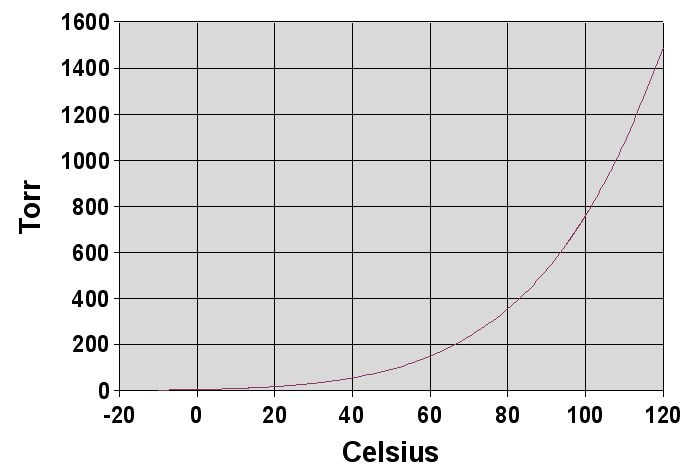
\includegraphics[width=10cm]{./figures/VaporP_1.png}
\caption{水的饱和蒸汽压, 横坐标是摄氏温度, 纵坐标是毫米汞柱(图片来自维基百科)} \label{VaporP_fig1}
\end{figure}

我们用一个函数 $P_\alpha(T)$ 描述饱和蒸汽压和温度的关系. 例如水蒸气的饱和蒸汽压记为 $P_{H2O}(T)$ (\autoref{VaporP_fig2}). 若容器的体积可以变化, 当容器变大而温度不变时, 压强首先会变小, 但液体会继续汽化, 直到压强恢复到饱和蒸汽压时重新达到平衡. 反之, 当容器体积变小(温度不变), 则压强首先升高,  然后气体会逐渐液化直到恢复饱和蒸汽压时重新达到平衡. 一般来说, 温度升高会导致饱和蒸汽压升高.

为了方便讨论, 我们以下假设蒸汽为理想气体\upref{PVnRT}. 在常温常压(或更低温低压)下这一般是近似成立的, 但在高温高压下假设会失效. 将饱和蒸汽压带入理想气体状态方程会发现饱和蒸汽的分子密度只于温度有关
\begin{equation}\label{VaporP_eq2}
\frac{n_\alpha}{V}  = \frac{P_\alpha(T)}{R T}
\end{equation}

\begin{exercise}{水蒸气的质量}
求 25°C 时一立方米饱和水蒸气的质量.
\end{exercise}

\subsection{混合气体}
\pentry{理想气体分压定律\upref{PartiP}}

我们接下来讨论容器中除了某种液体及其蒸汽外, 还有另一种气体的情况. 以水, 水蒸气和干燥的空气为例. 如果将两种气体都视为理想气体, 那么两种气体的总压强可以根据分压定律来计算, 即水蒸气单独存在时的压强加上空气单独存在时的压强. 另外, 假设空气分子不溶于水且不与水分子发生任何反应, 则水蒸气的分压仍然是 $P_{H2O}(T)$. 各种气体的分子密度仍然可以用\autoref{VaporP_eq2} 计算.

令干燥空气的分压为 $P_{air}$ 则混合气体总压强 $P$ 为
\begin{equation}
P = P_{H2O}(T) + P_{air}
\end{equation}
所以若已知总压强和温度, 根据\autoref{VaporP_eq2}, 平衡时两种气体的比例为
\begin{equation}\label{VaporP_eq1}
\frac{n_{H20}}{n_{air}} = \frac{P_{H2O}(T)}{P_{air}} = \frac{P_{H2O}(T)}{P - P_{H2O}(T)}
\end{equation}

\subsection{绝对湿度和相对湿度}
我们下面来介绍日常生活中经常使用的相对湿度. 我们先定义\textbf{绝对湿度}为 $n'_{H20}/n'_{air}$ 或者 $P'_{H20}/P'_{air}$, 这里使用一瞥表示实际上的比例而不是平衡时的比例(\autoref{VaporP_eq1}). 若 $P$ 表示大气压强, 那么\autoref{VaporP_eq1} 就是某温度和汽压下可能出现的最大绝对湿度. 因为如果实际湿度稍高于这个值, 空气中的水蒸气就会迅速凝结到空气中的尘埃上, 形成云或雾, 有或者直接凝结到物体表面形成水滴或霜.

另一方面, 空气中绝对湿度常常低于\autoref{VaporP_eq1} 的值, 即水和水蒸气处于不平衡的状态. 这是因为地表的水(江湖海, 土壤等)蒸发的速度有限, 且大气并不是长期处于恒温恒压状态.

我们把\textbf{相对湿度}定义为水蒸气的分子实际密度(或分压)除以当前温度下饱和水蒸气的分子密度(或分压). 即
\begin{equation}
\phi = \frac{n'_{H2O}}{n_{H2O}} = \frac{P'_{H20}}{P_{H2O}}
\end{equation}

\subsection{沸腾}
在\autoref{VaporP_eq1} 中, 如果我们实时调节容器的体积, 使容器中的气体始终保持某个固定的压强 $P$, 当温度不断升高时, 绝对湿度也会不断升高. 当 $P_{H2O}(T)$ 趋近 $P$ 时, 容器里面就几乎只有水蒸气了. 此时如果温度继续升高使 $P_{H2O}(T)$ 等于或略大于 $P$, 系统就无法保持平衡, 水会不断汽化, 使容器不断膨胀, 直到所有的水都变为水蒸气为止. 我们把这个过程叫做\textbf{沸腾}, 并定义满足
\begin{equation}
P_{H2O}(T_b) = P
\end{equation}
的温度 $T_b$ 为\textbf{沸点}. 注意沸点于液体的种类以及压强有关.
